\documentclass[runningheads,a4paper]{llncs}
\usepackage[T1]{fontenc}
\usepackage{lmodern}
\usepackage{graphicx}
\usepackage{amsmath, amssymb}
\usepackage{url}
\urlstyle{same}
\makeatletter
\g@addto@macro\UrlBreaks{\do\/\do\-\do\.\do\_\do\a\do\b\do\c\do\d\do\e\do\f
  \do\g\do\h\do\i\do\j\do\k\do\l\do\m\do\n\do\o\do\p\do\q\do\r\do\s\do\t
  \do\u\do\v\do\w\do\x\do\y\do\z\do\D\do\E\do\M\do\R\do\S\do\V}
\makeatother
\usepackage{booktabs}
\usepackage{xcolor}
\usepackage{tikz}
\usetikzlibrary{positioning,arrows.meta,calc,shadows,backgrounds,shapes.geometric}
\usepackage{cite}
\setlength{\emergencystretch}{2em}
\renewcommand{\topfraction}{0.95}
\renewcommand{\bottomfraction}{0.8}
\renewcommand{\textfraction}{0.1}
\renewcommand{\floatpagefraction}{0.95}
\setcounter{topnumber}{3}
\setcounter{totalnumber}{4}

\begin{document}

\title{Robust Emergency Vehicle Detection\\ with Audio-Visual Late Fusion:\\
A Benchmark and Diagnosis}
\titlerunning{Robust EV Detection with Audio-Visual Late Fusion}

\author{Vikash\inst{1} \and Yash Yadav\inst{2} \and Aman Singh\inst{1}
\and Madan Lal Saini\inst{1}}
\authorrunning{Vikash et al.}
\institute{Chandigarh University, Punjab, India
\and
Bennett University, Greater Noida, India}

\maketitle

\begin{abstract}
Emergency vehicle detection is often challenging in poor lighting, glare, bad
weather and heavy occlusion. Audio-visual models typically fuse the two
modalities with a fixed weight. We test whether a learned per-sample
reliability gate performs better than simple rules. We build three benchmarks
from public data: EV-AVSim-L, a leakage-free composite benchmark of 12,433
images, 8,637 UrbanSound8K audio clips and 28,000 pairs; VGGSound-EV, 9,155 real
audio-visual clips; and an out-of-source test in which neither the images nor
the audio of the test samples were seen during training. Late fusion gives a
large increase in performance, with AUPRC rising from 0.853 (vision) and 0.786
(audio) to 0.905--0.920. The visual $F_1$ drops to 0.15 in the strongest fog,
while all fusion rules keep a score of at least 0.54. The logistic and MLP
gates achieve 0.919 and 0.920 respectively, compared with 0.917 for the
parameter-free noisy-OR rule. However, on real clips the gates (0.974 and
0.970) bring no gain over noisy-OR (0.973), and on out-of-source clips they
perform worse than noisy-OR (0.892 against 0.905), although they are better
calibrated. The gate coefficients explain why: after temperature scaling,
most of the reliability information is already contained in the calibrated
confidence scores. An oracle gate achieves 0.985, showing that per-sample
selection could still bring improvements. The full system contains only
1.67\,M parameters.
\keywords{Emergency vehicle recognition \and Multimodal fusion \and
Modality reliability \and Confidence calibration \and Robustness.}
\end{abstract}

\section{Introduction}

Improved reliability in emergency vehicle detection can reduce response time
and help with pre-emptive traffic signalling \cite{su2022}. Visual models such
as CNNs, YOLO and transformers achieve good performance in clear conditions
\cite{hu2025}; however, they suffer in poor lighting, glare and occlusion
\cite{li2024,alam2024}. This is particularly problematic in Indian traffic
\cite{kumar2025}. Adding an audio channel can help, as the siren can be heard
even when the vehicle cannot be seen \cite{sun2021}. While most systems use a
fixed weight to fuse the modalities \cite{baltrusaitis2019,kittler1998}, the
quality of each modality varies with the lighting, weather and traffic.

We ask whether performance improves when a weight is learned for each sample.
Compared with our earlier study, we increase the image corpus by 7.6 times and
include real video clips with audio. Our contributions are:
\begin{itemize}
\item \textbf{Three benchmarks from public data:} EV-AVSim-L, a leakage-free
composite benchmark of 12,433 images, 8,637 audio clips and 28,000 pairs across
five scenarios; VGGSound-EV, 9,155 real audio-visual clips; and an
out-of-source test with near-duplicate removal.
\item \textbf{A controlled degradation experiment} with five visual and three
audio corruptions at five strengths, together with an analysis of naturally
dark real frames.
\item \textbf{A fair comparison of eleven fusion rules}, including logistic and
multi-layer perceptron (MLP) reliability gates, using three training and three
pairing seeds with bootstrap intervals and McNemar tests.
\item \textbf{A diagnosis} of why the learned gates give little improvement
over calibrated parameter-free rules (a small improvement on composite pairs,
none on real clips), with an oracle that shows the potential improvement from
per-sample selection.
\end{itemize}

\section{Related Work}

Vision-based emergency vehicle detection achieves good performance with YOLO
and RT-DETR style detectors in structured scenes \cite{hu2025}. However,
performance still suffers in poor lighting \cite{li2024}, glare \cite{alam2024}
and occlusion. Enhancement can help \cite{li2024}, but vehicles will not be
detected if they cannot be seen. Indian roads introduce additional issues
such as lighting changes at night, monsoon weather and mixed traffic; datasets
like DriveIndia capture these issues but are limited in size \cite{kumar2025}.

Audio-based emergency vehicle detection classifies the siren using MFCC or
log-Mel features and can be used in poor visibility \cite{sun2021}; recent work
runs siren detection in real time on embedded systems \cite{giordano2025}.
Early and late fusion can both improve robustness \cite{baltrusaitis2019}.
Recent emergency vehicle systems fuse the channels with a stacking ensemble of
a siren network and a YOLO detector \cite{zohaib2024}, with an edge system that
requires the camera and microphone to agree \cite{kristiawan2026}, or with a
distilled audio-visual transformer \cite{john2026}; all use a fixed decision
rule or weight. In the wider multimodal field there is strong interest in
fusing low-quality data \cite{zhang2024survey}, and dynamic fusion that gives
each modality a sample-dependent weight has been proposed with theoretical
guarantees \cite{cao2024}.

Care must also be taken in evaluation. If the image and audio corpora are
paired arbitrarily, the audio provides no information about the image. With
UrbanSound8K, randomly splitting the data inflates accuracy because slices
of the same recording end up in different splits; the 10 fixed folds avoid
this \cite{salamon2014}. Large public datasets now allow more realistic
benchmarks: Open Images \cite{kuznetsova2020} and ImageNet
\cite{russakovsky2015} contain thousands of human-labelled emergency vehicle
images, and VGGSound \cite{chen2020} contains real YouTube clips of sirens and
road traffic, selected so that the sound source is visible.

\section{Proposed Method}

Each sample consists of a video frame and a short audio clip, and the label
indicates whether an emergency vehicle is present (visible or not). Each
unimodal model provides a confidence score. Static late fusion combines the two
confidence scores with the same weight for all samples. However, the
reliability of each channel (the probability that its decision is correct)
changes with the scenario, so the weight should depend on the sample. This
requires the confidence scores to be comparable (\textbf{R1},
Sec.~\ref{sec:calib}), the weight to depend on the scenario (\textbf{R2},
Sec.~\ref{sec:gate}) and a principled way to combine the probabilistic
evidence (\textbf{R3}, Sec.~\ref{sec:pool}). The pipeline is shown in
Fig.~\ref{fig:architecture}.

@@FIG1@@

\subsection{Unimodal Recognisers}

The vision branch classifies the full image, as most of the images only have
image-level labels. We use MobileNetV3-Small \cite{howard2019} at
$224\times224$ with ImageNet initialisation, fine-tuned using binary
cross-entropy with random crops and horizontal flips. The audio branch uses a
4\,s window to compute a 64-band log-Mel spectrogram, which is classified by a
compact three-block CNN with at most 64 channels \cite{salamon2017}. The
network is trained with time and frequency masking \cite{park2019}, random
time shifts and a positive class weight.

\subsection{Confidence Calibration}
\label{sec:calib}

To make the confidence scores comparable (\textbf{R1}), each branch is
temperature scaled \cite{guo2017}: the logit is divided by a single scalar for
each modality, $\hat{p}_m = \sigma(\operatorname{logit}(p_m)/T_m)$ for
$m \in \{v, a\}$, fitted on the validation set using the negative
log-likelihood. This does not affect the AUROC or AUPRC of a branch, but it makes the
confidence scores comparable.

\subsection{Context-Dependent Reliability Gate}
\label{sec:gate}

To make the weight depend on the scenario (\textbf{R2}), a 17-dimensional
context descriptor $\phi(x)$ is computed without any extra network. It
contains 7 visual features (luminance, RMS contrast, Laplacian variance, dark
channel \cite{he2011}, saturated pixels, edge density and colourfulness), 6
audio features (RMS level, an SNR estimate based on frame energy, spectral
flatness, energy in the siren band of 0.5--1.8\,kHz, top-1\% energy share and
spectral centroid) and 4 confidence features (the two calibrated confidence
scores and their distances from 0.5). The gate returns a weight between 0.05
and 0.95 for the vision branch, $w_v(x)=0.05+0.9\,g(\phi(x))$, and the audio
weight is one minus the vision weight. We investigate two forms of the gate
$g$: a
logistic model with interpretable coefficients, and a multi-layer perceptron
(MLP) with one hidden layer of 32 units. Both are trained on the training
split to predict which modality was correct: the target is 1 if only the
vision branch was correct, 0 if only the audio branch was correct, and 0.5,
with a reduced weight, if both or neither were correct.

\subsection{Log-Odds Pooling}
\label{sec:pool}

To combine the confidence scores in a principled way (\textbf{R3}), the
calibrated confidence scores are pooled in log-odds space \cite{kittler1998}:
\begin{equation}
s(x) = \sigma\!\Big( w_v(x)\,\operatorname{logit}(\hat p_v)
                   + w_a(x)\,\operatorname{logit}(\hat p_a) + b \Big),
\label{eq:pool}
\end{equation}
where the bias $b$ is fitted on the validation set, and a detection is made if
the score is above a threshold $\tau$. As the weights sum to one,
Eq.~(\ref{eq:pool}) is a weighted average of the log-odds: if one branch is
confident (its logit is far from zero), it dominates the other, and the bias
re-calibrates the score. However, this does not combine independent
evidence: if both branches give a confidence of 0.8, the score is still 0.8
when $b=0$. The noisy-OR rule does combine evidence in this way, so we use it
as our main baseline.

\section{Benchmarks and Data}
\label{sec:pairing}

\textbf{Images.} We use 1,244 images from Open Images V7
\cite{kuznetsova2020} with verified annotations of an ambulance, fire
apparatus, police car or emergency vehicle, and 1,896 negatives: hard
negatives verified not to contain an emergency vehicle but containing a car,
truck, bus, van or taxi, and further vehicle images. We also use the
ambulance, fire engine and police van classes of ImageNet
\cite{russakovsky2015} (4,050 positives) and 15 classes of ordinary vehicles
(5,243 negatives). The images are split 70/15/15, stratified by source and
label, giving 8,703/1,865/1,865 images.

\textbf{EV-AVSim-L (composite).} Each sample combines one image with one
UrbanSound8K clip. The samples cover five scenarios with fixed proportions:
S1 (20\%) EV visible and siren, S2 (15\%) EV visible and non-siren audio, S3
(15\%) no EV visible and siren, S4 (30\%) no EV and no siren, and S5 (20\%)
no EV and a confusable sound (horn, engine or street music). S1--S3 are
positive. S2 and S3 contain conflicting evidence from the two modalities,
which separates the fusion rules. The audio uses the official folds 1--8/9/10
for training/validation/testing; we remove the 95 slices of the single
recording that crosses this boundary, and we assert in our code that no
recording, image or clip appears in two splits. The pairs are generated within
each split (20,000/4,000/4,000) with a positive rate of 0.50 and three pairing
seeds.

\textbf{VGGSound-EV (real).} The clips are 10\,s YouTube videos whose sound
source was selected to be visible on screen \cite{chen2020}. We downloaded,
from a public mirror, the clips of the classes ambulance siren, fire truck
siren and police car siren (positives), and car passing by, driving buses,
driving motorcycle, car engine idling, engine revving, vehicle horn and civil
defence siren (negatives; the civil defence siren is a siren without an
emergency vehicle). We use the frame at 5\,s and the audio from 3 to 7\,s, so
that both come from the same moment. The data is split into video-disjoint
splits (one split per YouTube ID), giving 5,487/1,834/1,834 clips with a
positive rate of 33\%. The task on this benchmark is to detect emergency
events (an emergency vehicle sounding its siren), whereas on EV-AVSim-L a
sample is positive if the vehicle is visible, the siren can be heard, or both.
Neither benchmark tests visual recognition alone. The audio branch is trained
on UrbanSound8K folds 1--8 together with the VGGSound-EV training clips.

\textbf{Out-of-source (OOD).} To test generalisation, we retrain both
branches from scratch using only ImageNet and UrbanSound8K (same splits and
settings, 3 seeds), and fit the calibration, gates and thresholds on composite
ImageNet and UrbanSound8K pairs. The Open Images photos and the VGGSound audio
and frames are never used for training, model selection or thresholds. We test
on (i) 4,000 composite pairs of Open Images and VGGSound audio (same five
scenarios) and (ii) 8,592 real VGGSound-EV clips. We first remove near
duplicates of the training data: 11 images and 7 frames within a dHash
distance of 4 bits of an ImageNet image, and, conservatively, 556 clips whose
coarse log-Mel fingerprint has a cosine similarity of at least 0.98 with an
UrbanSound8K clip.

\textbf{Degradation.} Following \cite{hendrycks2019}, we apply five visual
corruptions at five strengths: low light (gamma and Poisson--Gaussian noise),
fog (Koschmieder atmospheric scattering model \cite{narasimhan2002}), rain,
motion blur and glare. For audio we add broadband traffic-like noise (SNR 20,
10, 5, 0 and $-5$\,dB), low-frequency wind buffeting and clipping. The models
are trained without corruption.

\section{Experimental Setup}
\label{sec:setup}

The vision branch is fine-tuned with the AdamW variant of Adam
\cite{kingma2015}, using a weight decay of $10^{-4}$, a learning rate of
$3\times10^{-4}$, a batch size of 32 and a cosine schedule, for up to 12 epochs
with early stopping after 4 epochs without improvement. The audio branch is
trained for 30 epochs with a learning rate of $2\times10^{-3}$ and a batch
size of 64. The checkpoint with the best validation AP is kept. The
temperatures, bias, gates, static weight and all thresholds are fitted using
only the training and validation data, and the test data is used only once.
Both branches are trained with @@nseeds@@ seeds, and all numbers are the mean
and standard deviation across the seeds. For the main comparison between the
gates and noisy-OR we also give 95\% confidence intervals of the difference in
AUPRC, calculated from 1000 clustered bootstrap resamples \cite{efron1993} of
source images and clips (composite pairs) or whole videos (real clips),
because pairs share sources. The full
study ran on a two-core CPU. Results are reported as AUPRC (main metric), AUROC, $F_1$ at
the validation threshold and recall at 10\% FPR. Exact McNemar tests
\cite{dietterich1998} are performed between each gate and noisy-OR at the
validation thresholds, with Holm correction over all @@ntests@@ tests. The
baselines use the same calibrated confidence scores: vision only, audio only,
mean, max, noisy-OR $1-(1-\hat p_v)(1-\hat p_a)$, static weighted (grid search
for the vision weight), learned late fusion (logistic regression on both
calibrated confidence scores), the hand-crafted context rules of our previous
system, and an oracle that picks the correct modality for each sample. A gate
must outperform noisy-OR to claim any contribution, because combining two
detectors already improves recall.

\begin{table}[htbp]
\centering
\caption{EV-AVSim-L test results (4,000 pairs, pairing seed 42), mean $\pm$
s.d.\ over @@nseeds@@ seeds. Bold: best non-oracle value.}
\label{tab:main}
\scriptsize
\setlength{\tabcolsep}{5pt}
\begin{tabular}{lcccc}
\toprule
Method & AUPRC & AUROC & $F_1$ & Recall@FPR 0.1 \\
\midrule
@@tab.syn@@
\bottomrule
\end{tabular}
\end{table}

\section{Results and Analysis}
\label{sec:results}

\textbf{Confidence calibration.} Both branches are over-confident. After
temperature scaling ($T_v = @@T.syn.v@@$, $T_a = @@T.syn.a@@$), the validation
ECE drops from @@ece0.syn.v@@ to @@ece1.syn.v@@ for vision and from
@@ece0.syn.a@@ to @@ece1.syn.a@@ for audio.

\textbf{Composite benchmark.} All late fusion rules greatly improve
performance (Table~\ref{tab:main}). The AUPRC increases from 0.853 (vision) and
0.786 (audio) to 0.905--0.920, and the recall at 10\% FPR from 0.623 (vision)
and 0.426 (audio) to 0.716--0.763. The logistic gate (0.919) and the MLP gate
(0.920) perform just better than noisy-OR (0.917) and max fusion (0.917).
Across all three pairing seeds the gates outperform noisy-OR by 0.001--0.006
AUPRC, but all confidence intervals include zero (Table~\ref{tab:stats}).
After Holm correction, the logistic gate makes significantly fewer errors than
noisy-OR in @@h.syn.log.win@@ of @@nruns@@ seed/pairing runs and the MLP gate in
@@h.syn.mlp.win@@ of @@nruns@@ (and never more). The learned gates therefore
give a small improvement on the composite pairs, which comes from a better
operating point rather than a better ranking.

\textbf{Real audio-visual clips.} On VGGSound-EV we fit the fusion either on
the real clips (in-domain) or on EV-AVSim-L (zero-shot) (Table~\ref{tab:real}).
The audio branch performs well (AUPRC 0.969), but the vision branch performs
poorly (0.642), as the vehicle is often not clearly visible in the sampled
frame. Noisy-OR (0.973) gives a slight improvement over the audio branch
alone, and neither the logistic gate (0.974) nor the MLP gate (0.970) improves
on it. As the confidence intervals include zero, there is no significant
improvement from the gates, and the logistic gate is significantly worse than
noisy-OR in @@h.ind.log.loss@@ of @@nseeds@@ seeds. The AUPRC remains similar in
the zero-shot setting (noisy-OR 0.967, logistic gate 0.964, MLP gate 0.963),
which shows that the fusion learned on composite pairs generalises to real
clips. Here the gates rank slightly worse than noisy-OR, but because the
transferred noisy-OR threshold fits poorly ($F_1$ 0.887), the logistic gate
makes fewer errors than noisy-OR in @@h.zs.log.win@@ seed and the MLP gate in
@@h.zs.mlp.win@@ seeds. The oracle (0.996) shows that a better per-sample choice
could remove most of the remaining errors.

\begin{table}[htbp]
\centering
\caption{VGGSound-EV test results (1,834 real clips), mean $\pm$ s.d.\ over
@@nseeds@@ seeds; fusion fitted on VGGSound-EV (in-domain) or EV-AVSim-L
(zero-shot). Bold: best non-oracle value.}
\label{tab:real}
\resizebox{\textwidth}{!}{%
\begin{tabular}{lcccccc}
\toprule
 & \multicolumn{3}{c}{In-domain} & \multicolumn{3}{c}{Zero-shot} \\
\cmidrule(lr){2-4}\cmidrule(lr){5-7}
Method & AUPRC & $F_1$ & R@FPR 0.1 & AUPRC & $F_1$ & R@FPR 0.1 \\
\midrule
@@tab.real@@
\bottomrule
\end{tabular}}
\end{table}

\begin{table}[htbp]
\centering
\caption{Gate minus noisy-OR AUPRC (95\% clustered-bootstrap CI) and seeds
with significantly fewer/more errors (W/L, Holm-corrected McNemar).}
\label{tab:stats}
\scriptsize
\setlength{\tabcolsep}{2pt}
\begin{tabular}{lcccc}
\toprule
Benchmark & Logistic $\Delta$AUPRC [95\% CI] & W/L & MLP $\Delta$AUPRC [95\% CI] & W/L \\
\midrule
@@tab.stats@@
\bottomrule
\end{tabular}
\end{table}

\textbf{Out-of-source.} The source shift has a clear effect
(Table~\ref{tab:ood}). The vision branch drops from an AUPRC of 0.958 on
held-out ImageNet images to 0.757 on Open Images photos. The audio branch
performs well on VGGSound audio (0.895), and reaches 0.594 on UrbanSound8K
fold 10, which contains only 83 siren slices. Fusion still helps: on the
out-of-source composite pairs, noisy-OR (0.889) outperforms the vision branch
(0.743) and the audio branch (0.837). However, the order of the fusion rules
changes. In domain, the gates perform best (0.927 and 0.928, against 0.918 for
noisy-OR); on out-of-source samples they underperform noisy-OR, and the
confidence intervals of the difference exclude zero (Table~\ref{tab:stats}).
A gate trained on one set of sources therefore generalises worse than the
parameter-free rule. However, the learned rules are better calibrated under
the source shift: on real clips the logistic gate has an ECE of 0.179 and
learned late fusion 0.123, whereas noisy-OR has 0.289, and the Brier score of
the logistic gate is 0.125 against 0.198 for noisy-OR. Their probabilities are
therefore more trustworthy, even though their ranking is worse.

\begin{table}[htbp]
\centering
\caption{Out-of-source test (training on ImageNet and UrbanSound8K only, mean
over @@nseeds_ood@@ seeds). ID: ImageNet--UrbanSound8K pairs; OOD-C: Open
Images--VGGSound pairs; OOD-R: real VGGSound-EV clips. Bold: best value.}
\label{tab:ood}
\resizebox{\textwidth}{!}{%
\begin{tabular}{lccccccc}
\toprule
 & ID & OOD-C & \multicolumn{5}{c}{OOD-R} \\
\cmidrule(lr){2-2}\cmidrule(lr){3-3}\cmidrule(lr){4-8}
Method & AUPRC & AUPRC & AUPRC & $F_1$ & FPR & ECE & Brier \\
\midrule
@@tab.ood@@
\bottomrule
\end{tabular}}
\end{table}

\textbf{Robustness.} Under synthetic corruption (Fig.~\ref{fig:degradation}),
the vision $F_1$ drops from 0.73 to 0.15 in the strongest fog and to 0.60 in
the strongest glare, while every fusion rule keeps an $F_1$ of at least 0.54.
The audio $F_1$ drops from 0.54 to 0.36 in the strongest traffic noise, while
the fusion rules stay at 0.78 or more. The gate's mean vision weight moves in the
correct direction (0.57 clean, 0.40 in dense fog, 0.64 in loud noise), but at
high visual severity its clean-data threshold no longer fits, so its $F_1$
drops below that of the static rule. On naturally dark real frames (mean luminance
below 0.25; 207 clips), the vision AUPRC drops to 0.549 (0.655 on the other
frames), whereas noisy-OR (0.978) and the logistic gate (0.981) are
unaffected.

\begin{figure}[htbp]
\centering
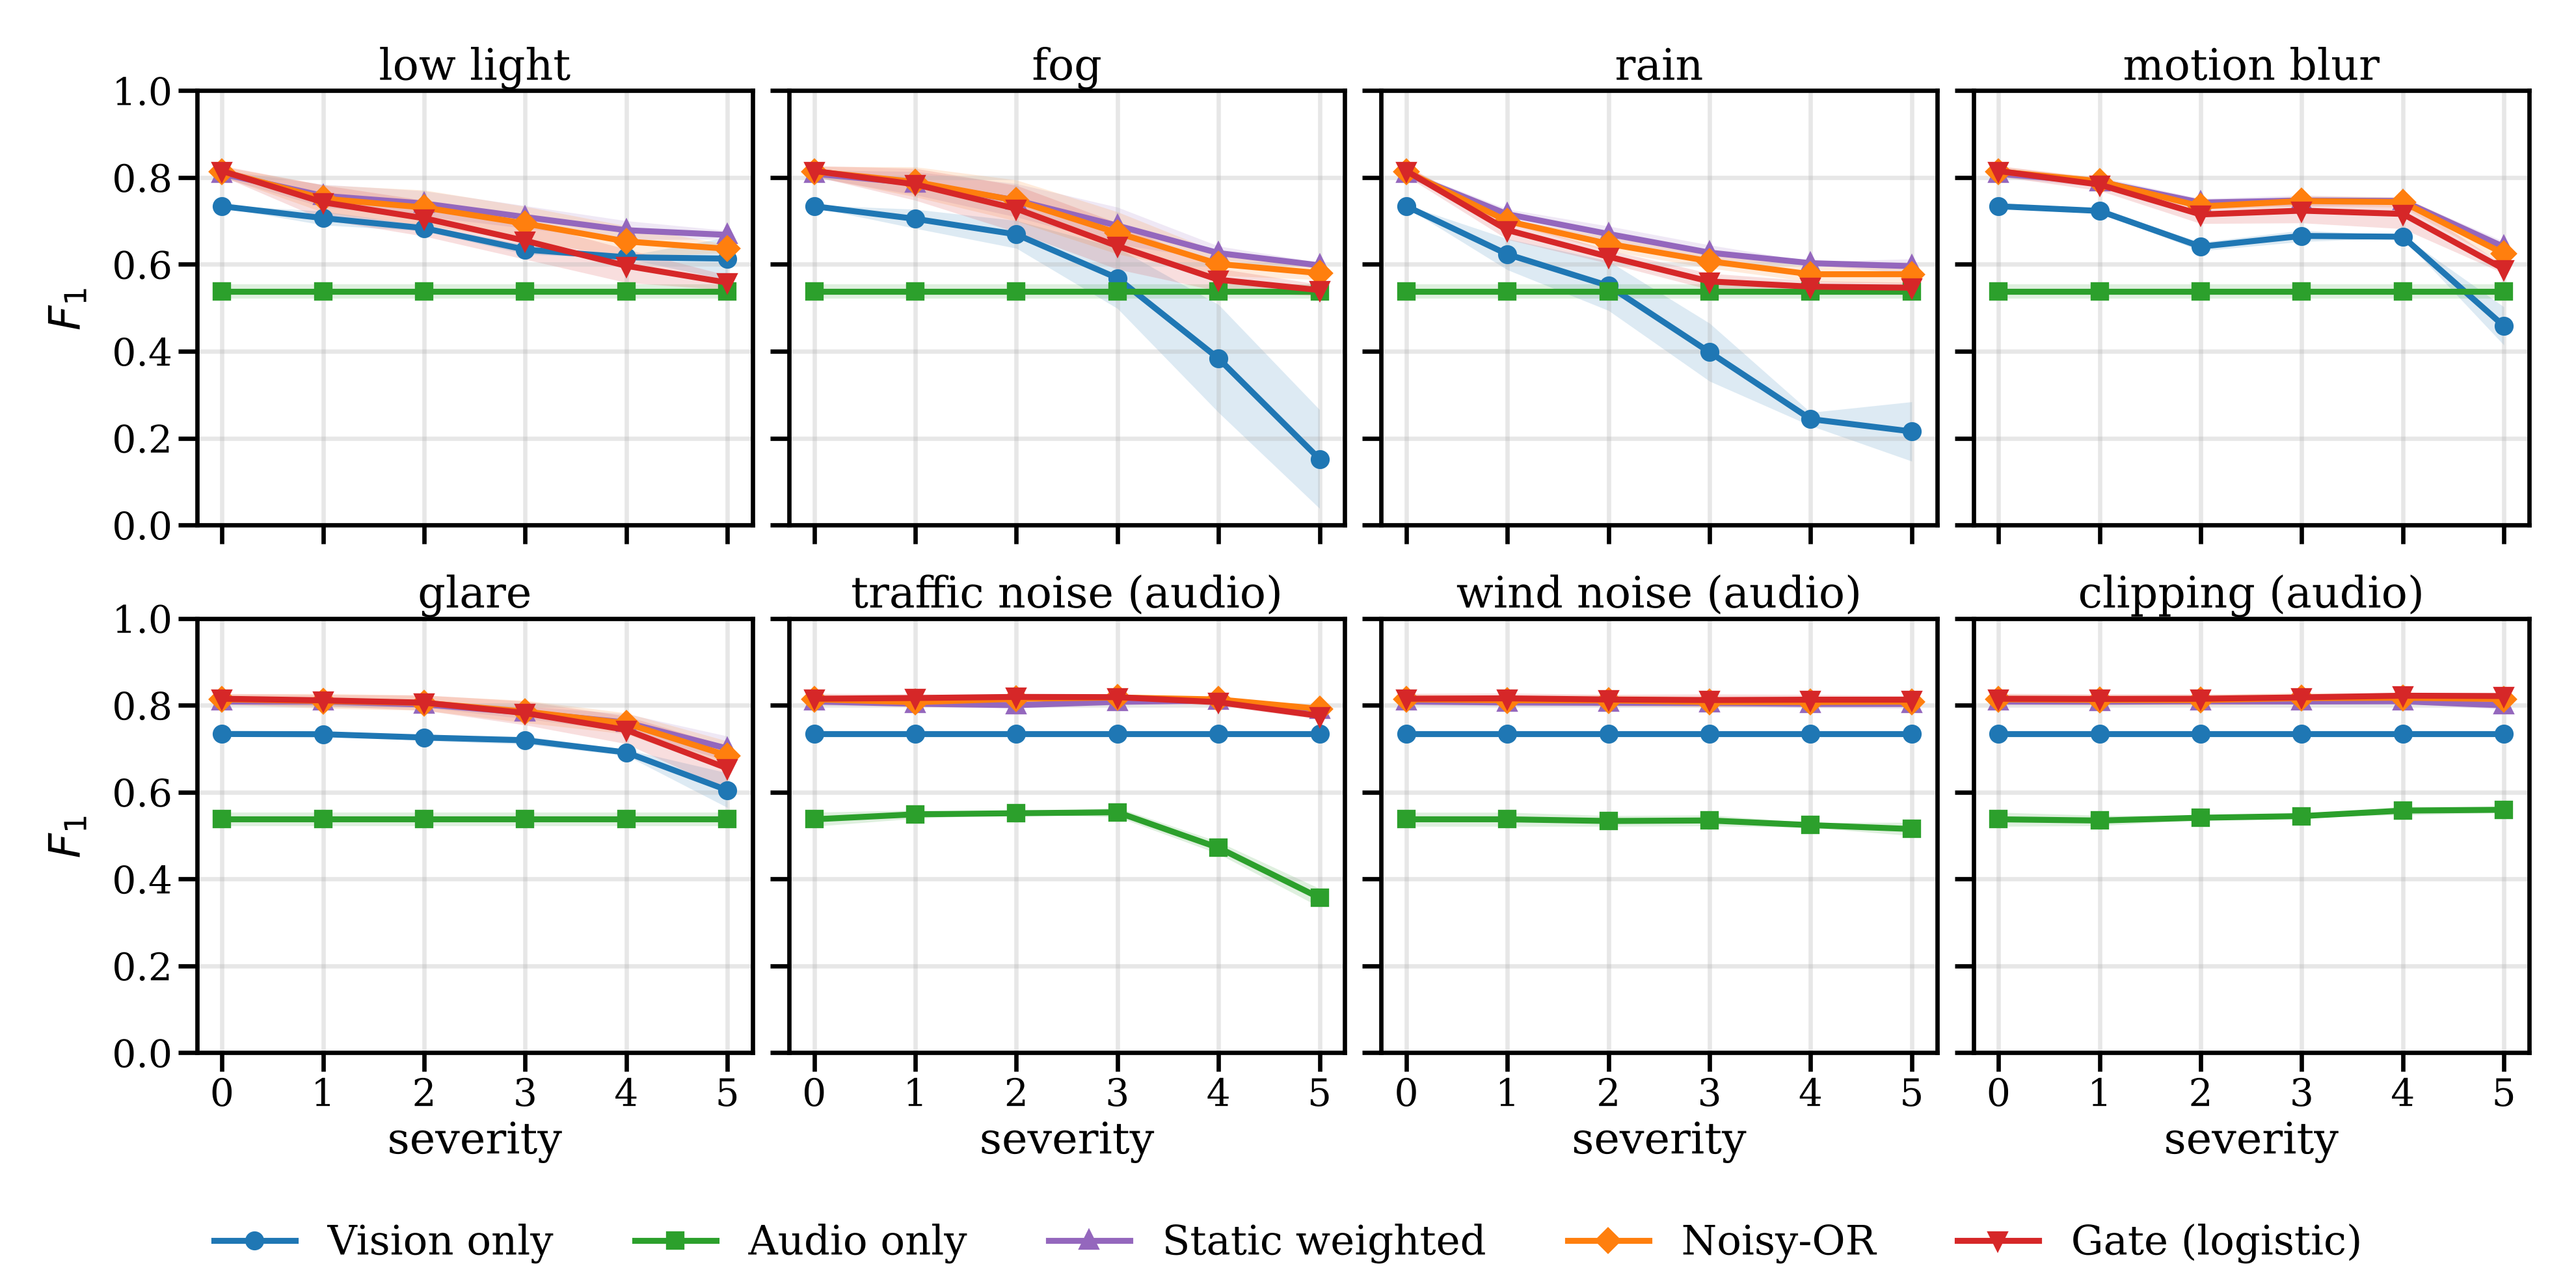
\includegraphics[width=0.72\textwidth]{degradation_curves_v4.png}
\caption{Test $F_1$ on EV-AVSim-L against corruption severity (0 = clean;
mean $\pm$ s.d.\ over @@sw.n@@ seeds). Top: visual; bottom: audio corruptions.}
\label{fig:degradation}
\end{figure}

\textbf{Gate behaviour.} The logistic gate coefficients on standardised
features (mean over @@nseeds@@ seeds) explain the main result. The calibrated
confidence scores have the largest coefficients ($+1.60$ and $-1.52$),
followed by the margins, while none of the image or audio quality features has
a coefficient above 0.16 in magnitude. The gate therefore mostly reuses what
noisy-OR already uses. On real clips, luminance ($+0.23$) and the dark channel
($-0.22$) receive some weight, so the gate trusts the camera less in dark
frames, but this changes few decisions.

\section{Discussion}

Our results show that late fusion is clearly more robust than either branch:
it increases AUPRC by 0.05--0.07 on composite pairs and keeps working when the
camera fails. A learned sample-dependent weight, however, adds little: the
gates beat noisy-OR by at most 0.006 AUPRC on composite pairs, do not improve
on real co-recorded clips and underperform on out-of-source data, which
suggests that they partly fit the training sources.

The reason is that calibrated confidences already carry most of the
reliability information. In fog, the vision branch already returns a
confidence of about 0.5, so a descriptor only helps if it predicts a branch's
errors beyond its confidence, and ours mostly do not. We recommend always reporting a calibrated noisy-OR baseline and an
oracle gate; the oracle (0.985, against 0.920 for the best practical rule)
shows what better reliability signals could bring.

\section{Practical and Societal Impact}

\textbf{Practical implications.} Our findings suggest a simple solution in
which both branches are calibrated and combined with a fixed rule such as
noisy-OR. It needs no gate training, matched the gates on real clips, was within 0.006
AUPRC of them on composite pairs and outperformed them on out-of-source data.
With 1.67\,M parameters and 82.6\,M MACs, it can run on low-cost edge devices
at junctions or inside vehicles. \textbf{Real-world applications.} The system could trigger traffic signal
pre-emption, send alerts to drivers through connected-vehicle messages, and
warn driver-assistance systems before an ambulance or fire engine can be
seen. \textbf{Societal benefits.} Quicker clearance of emergency vehicles leads to
faster response times in busy, mixed traffic such as on Indian roads, and the
low cost makes the system affordable for smaller cities. A deployment must not
store speech and should first be validated on local data
(Sec.~\ref{sec:limitations}).

\section{Limitations}
\label{sec:limitations}

\textbf{Data.} EV-AVSim-L pairs lack real-world correlations such as the
Doppler shift. VGGSound-EV labels only describe the sound (a positive clip may
not show the vehicle), it has no positive clips without a siren, and YouTube
favours clearer recordings. The corruptions are synthetic,
the dark-frame analysis uses a luminance threshold, none of our data was
recorded in India, and the classifiers cannot locate the vehicle to a lane.

\textbf{Method and evaluation.} We only tested two gates with hand-crafted
descriptors; a jointly trained network may find signals we missed, so we do
not claim that no gate can work. Three seeds capture only part of the training
variance, and the thresholds were chosen on clean validation data. The out-of-source test covers one direction (ImageNet
and UrbanSound8K to Open Images and VGGSound), and the duplicate filters are
heuristic.

\section{Conclusion and Future Work}

With more data, real clips and tests on unseen sources, we have confirmed that
late fusion clearly helps to detect emergency vehicles when a sensor fails.
Learned sample-specific gates gave only a small, non-significant improvement
over calibrated noisy-OR on composite pairs (0.920 against 0.917), no
improvement on real clips (0.974 against 0.973), and lower performance on
out-of-source data (0.892 against 0.905). This is because, once the confidence
scores are calibrated, the gate mostly reuses them. An open question is how to
learn more about a branch's reliability than its confidence shows; future work will look for such signals (for example, ensemble
disagreement), add localisation, and collect co-recorded data at junctions in
India.

\subsubsection*{Code and data availability.}
The code is available at
\url{https://github.com/vicky123411/Dynamic-Modality-Switching-for-Robust-Emergency-Vehicle-Detection}.
No dataset has been redistributed.


@@BIB@@
\end{document}

